\section{Feature Extraction}
As demonstrated by \cite{Raza_Mehmood_Ullah_Ahmad_Choi_On_2019} and \cite{Chen_Sun_Chen_Xie_Wu_Xu_2021}, MFCCs 
are highly effective features for heartbeat classification. In addition to MFCCs, 
we incorporated other features to capture various characteristics of heart sounds, enhancing the classification accuracy.
The features used are explained in the following section.

\subsection{Features Type}

\textbf{MFCC}\newline
Mel-Frequency Cepstral Coefficients (MFCCs) are representations of the short-term power spectrum of sound. 
They are derived by taking the Fourier transform of a signal, mapping the powers of the spectrum onto the mel 
scale, taking the logarithm, and then performing a discrete cosine transform. MFCCs are effective in capturing 
the timbral texture of audio and are widely used in speech and audio processing due to 
their ability to represent the envelope of the time power spectrum.
In heartbeat classification, MFFCs can reflect the different perceived quality of heart sounds,
such as the presence of murmurs or other anomalies.

\vspace{0.5cm}\noindent
\textbf{Chroma STFT}\newline
Chroma features represent the 12 different pitch classes of music (e.g., C, C\#, D, etc.). 
They are particularly useful for capturing harmonic and melodic characteristics in music. 
By mapping audio signals onto the chroma scale, these features can identify pitches regardless 
of the octave, making them useful for analyzing harmonic content in heart sounds.

\vspace{0.5cm}\noindent
\textbf{RMS}\newline
Root Mean Square (RMS) measures the magnitude of varying quantities, in this case, 
the amplitude of an audio signal. It is a straightforward way to compute the energy of 
the signal over a given time frame. RMS is useful in audio analysis for detecting volume 
changes and can help identify different types of heartbeats based on their energy levels.
For example, in a given timeframe the RMS may be altered by the presence of a murmur
with respect to a normal heart sound.

\vspace{0.5cm}\noindent
\textbf{ZCR}\newline
Zero-Crossing Rate (ZCR) is the rate at which a signal changes sign, indicating how often the signal 
crosses the zero amplitude line. It is particularly useful for detecting the noisiness and the temporal 
structure of the signal. In heartbeat classification, ZCR can help differentiate between normal and abnormal 
sounds by highlighting changes in signal periodicity.

\vspace{0.5cm}\noindent
\textbf{CQT}\newline
Constant-Q Transform (CQT) is a time-frequency representation with a logarithmic frequency scale, making it 
suitable for musical applications. Since it captures more detail at lower frequencies, it may be useful for analyzing 
the low-frequency components of heart sounds.

\vspace{0.5cm}\noindent
\textbf{Spectral Centroid}\newline
The spectral centroid indicates the center of mass of the spectrum and is often perceived as the brightness of a 
sound. It is calculated as the weighted mean of the frequencies present in the signal, with their magnitudes as 
weights. In heart sound analysis, a higher spectral centroid can indicate sharper, more pronounced sounds, 
while a lower centroid suggests smoother sounds. 

\vspace{0.5cm}\noindent
\textbf{Spectral Bandwidth}\newline
Spectral bandwidth measures the width of the spectrum around the centroid, providing an indication of the range 
of frequencies present. It is calculated as the square root of the variance of the spectrum. This feature helps 
in understanding the spread of the frequency components in the heart sounds, which can be indicative of different 
heart conditions.

\vspace{0.5cm}\noindent
\textbf{Spectral Roll-off}
Spectral roll-off is the frequency below which a certain percentage of the total spectral energy lies. It is 
typically set at 85\% and helps distinguish between harmonic and non-harmonic content. In heartbeat classification, 
spectral roll-off can be used to differentiate between sounds with a concentrated energy distribution and those with more dispersed energy.

\subsection{Methodology}
We extracted the features from the audio signals using the \textit{Librosa} library in Python. It is worth to underline four main aspects in the extraction
methodology having a direct impact on the results:
\begin{itemize}[leftmargin=*]
    \item \textbf{Normalization}: the audio are loaded using the \textit{torchaudio.load()} function, which normalized the audio signals in the range [-1, 1]. This is important to ensure that the features are on the same scale and to prevent the model from being biased towards features with larger values.
    \item \textbf{Audio Segmentation}: to extract features, we divided the audio recordings into chunks of a given length (in seconds). This segmentation allowed us to analyze the impact of different extraction intervals on model performance, additionally it allow for augmenting the data available. 
    \item \textbf{Sampling Rate}: while literature on spoken language often suggests that 16000 Hz is sufficient, it was necessary to assess the best sampling rate for heartbeat sounds specifically. We evaluated two sampling rates to determine the optimal rate for heartbeat sounds. 
    \item \textbf{Hop and Window Size}: the hop size determines the number of samples between successive windows, while the window size determines the number of samples considered. Each feature was extracted using the same window length and hop length facilitating a fair assessment of each feature's contribution to the classification task. 
\end{itemize}
The library used for the extraction is \textit{Librosa}, which is a Python package for music and audio analysis. 

\subsection{Sample Rate and Interval Selection}


\section{Methodology}

\subsection{Sampling Rate and Interval Choice}

\textbf{Experimental Setup}\newline
We trained various models (Random Forest, Support Vector Machine, Logistic Regression) with different features (Chroma, MFCC\_30, MFCC\_120, CQT\_30, CQT\_70),
sampling rates (mixed, 4000 Hz), and extraction intervals (0.5s, 1s, 2s, 3s). Features were used as extracted without any additional processing. 
The models were trained on 80\% of the data and tested on the remaining 20\%.

\subsubsection{Findings on Sampling Rate}
Our experiments revealed no clear advantage of using a mix of frequencies over a fixed sample rate, independently of the metric used.
Specifically, a fixed sampling rate of 4000 Hz was found to reduce the risk of bias introduction, improve efficiency, 
and enable the use of a wider variety of features. This sampling rate provided a consistent and reliable basis 
for feature extraction, as demonstrated in Figure \ref{fig:sample_rate_impact}.

\begin{figure}[H]
    \centering
    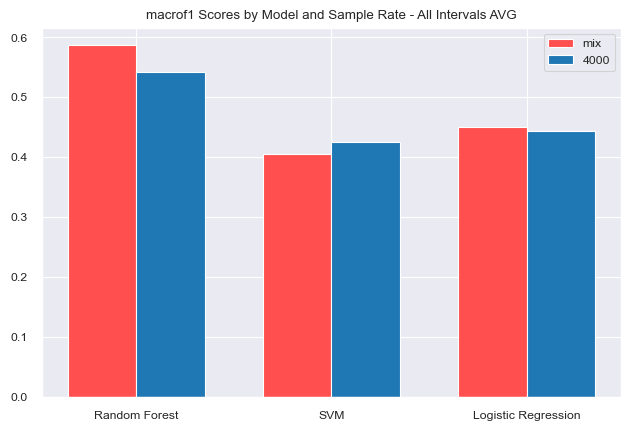
\includegraphics[width=1\columnwidth]{./images/sample_rate_impact.png}
    \caption{Comparison of the macro F1 score for different sampling rates.}
    \label{fig:sample_rate_impact}
\end{figure}

\subsubsection{Findings on Extraction Interval}
The choice of extraction interval had a significant impact on the number of samples and the class distribution, as shown in Figure \ref{fig:interval_class_distribution}.
To address the high class imbalance, we used the macro F1 score and Matthews Correlation Coefficient (MCC) as evaluation metrics. 
Our results indicated that a 2-second interval yielded the best performance. However, this choice also reduced the number of samples, 
potentially causing issues during training and testing, especially with more complex models. 

\begin{figure*}[htbp]
    \centering
    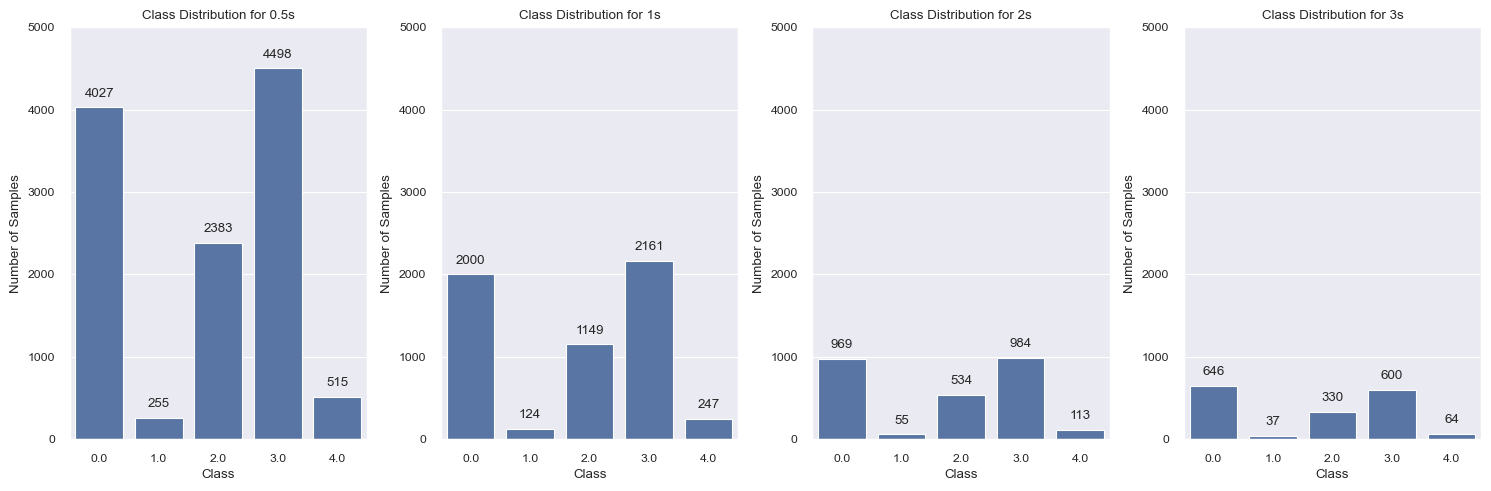
\includegraphics[width=1\textwidth]{./images/interval_class_distribution.png}
    \caption{Class distribution for different extraction intervals.}
    \label{fig:interval_class_distribution}
\end{figure*}

As a compromise, we recommend using a 1-second interval. This interval offers a good balance between 
the number of samples and the class distribution, ensuring robust model performance while maintaining a 
sufficient dataset size. Figures \ref{fig:interval_impact_macrof1} and \ref{fig:interval_impact_mcc} illustrate the impact of 
different extraction intervals on the macro F1 score and MCC, respectively.

\begin{figure}[H]
    \centering
    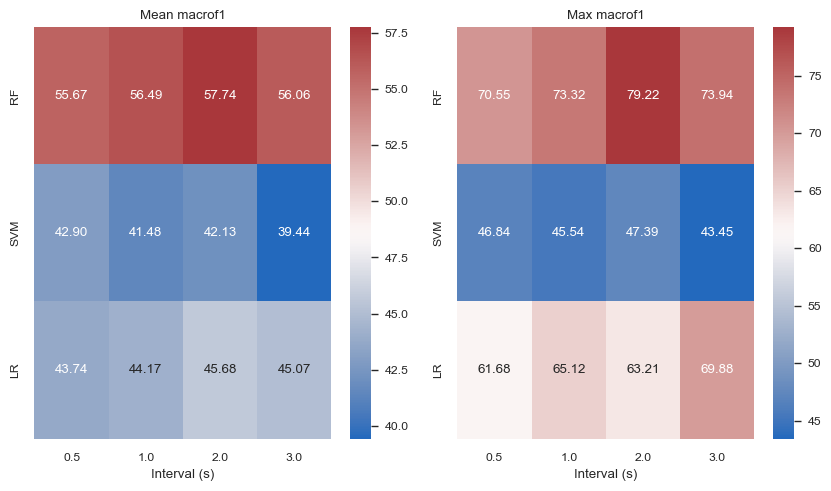
\includegraphics[width=1\columnwidth]{./images/interval_impact_macrof1.png}
    \caption{Comparison of the macro F1 score for different extraction intervals.}
    \label{fig:interval_impact_macrof1}
\end{figure}

\begin{figure}[H]
    \centering
    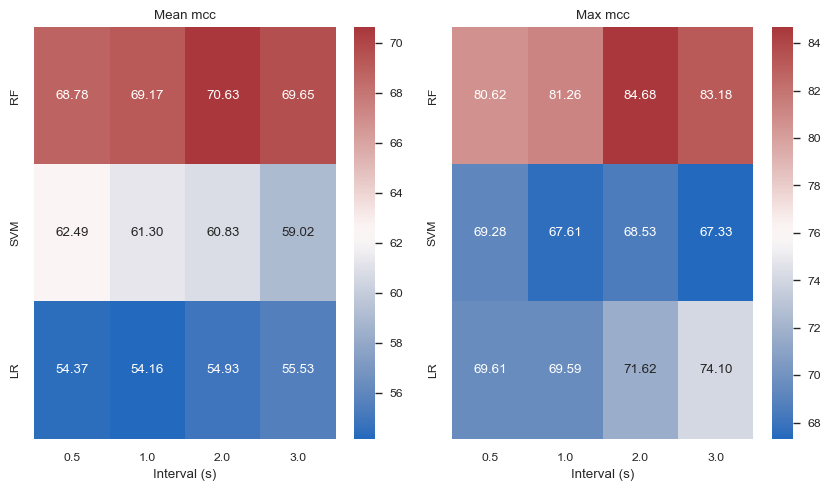
\includegraphics[width=1\columnwidth]{./images/interval_impact_mcc.png}
    \caption{Comparison of the MCC for different extraction intervals.}
    \label{fig:interval_impact_mcc}
\end{figure}


\subsection{Results}

